%%%%%%%%%%%%%%%%%%%%%%%%%%%%%%%%%%%%%%%%%%%%%%%%%%%%%%%%%%%%%%%%%%%%%%%%
%                                                                      %
%     File: Experimental.tex	                                       %
%     Tex Master: Thesis.tex                                           %
%                                                                      %
%     Author: Israel Sother                                            %
%     Last modified: 27 May 2024                                       %
%                                                                      %
%%%%%%%%%%%%%%%%%%%%%%%%%%%%%%%%%%%%%%%%%%%%%%%%%%%%%%%%%%%%%%%%%%%%%%%%
\section{Experimental Results}
\label{section:experimental}%chktex 24
\vfill

To validate the simulated results, some tests were made on a test bench. The \gls{rush} was implemented using Xilinx Model Composer inside Simulink, compared with the simulation implementation and then generated for the \gls{fpga} present in a Digilent Zybo Z7-20. The hardware used was comprised of the inverter developed on~\cite{Costa:MSc}, coupled with a current measuring board, developed for this thesis to increase noise immunity. This pairing was supplied with a power supply by Elektro-Automatik (EA-PSI 8360-15 DT) capable of up to 1.5kWh, and the characterized AMK motor was set in a test bench with a Sensor Technology torque transducer (RWT441-EC-PG) and another AMK motor as load. The complete setup is shown in \Cref{fig:testbench_steup}.

The inverter used in the experimental setup was a limiting factor due to the chosen semiconductors not being able to handle the maximum motor current. This limitation was explained in~\cite{Costa:MSc}, where it was mentioned that the intended mosfet was not available, thus an alternative semiconductor had to be used. The evolution of the SiC semiconductors since the previous design was also noticeable, going from a second SiC mosfet generation to a fourth, improving reliability and efficiency. Those limitations, combined with the advances in the SiC semiconductors industry exposed the need for a new hardware version. Even though this work focuses on the controller development, not the hardware, a new inverter design was made, covering the limitations of the current one. This new inverter design was not ready for the experimental tests, but a brief chapter on the design process is included in \Cref{chapter:appendix_inverter}.

\begin{figure}[!htb]
	\centering
	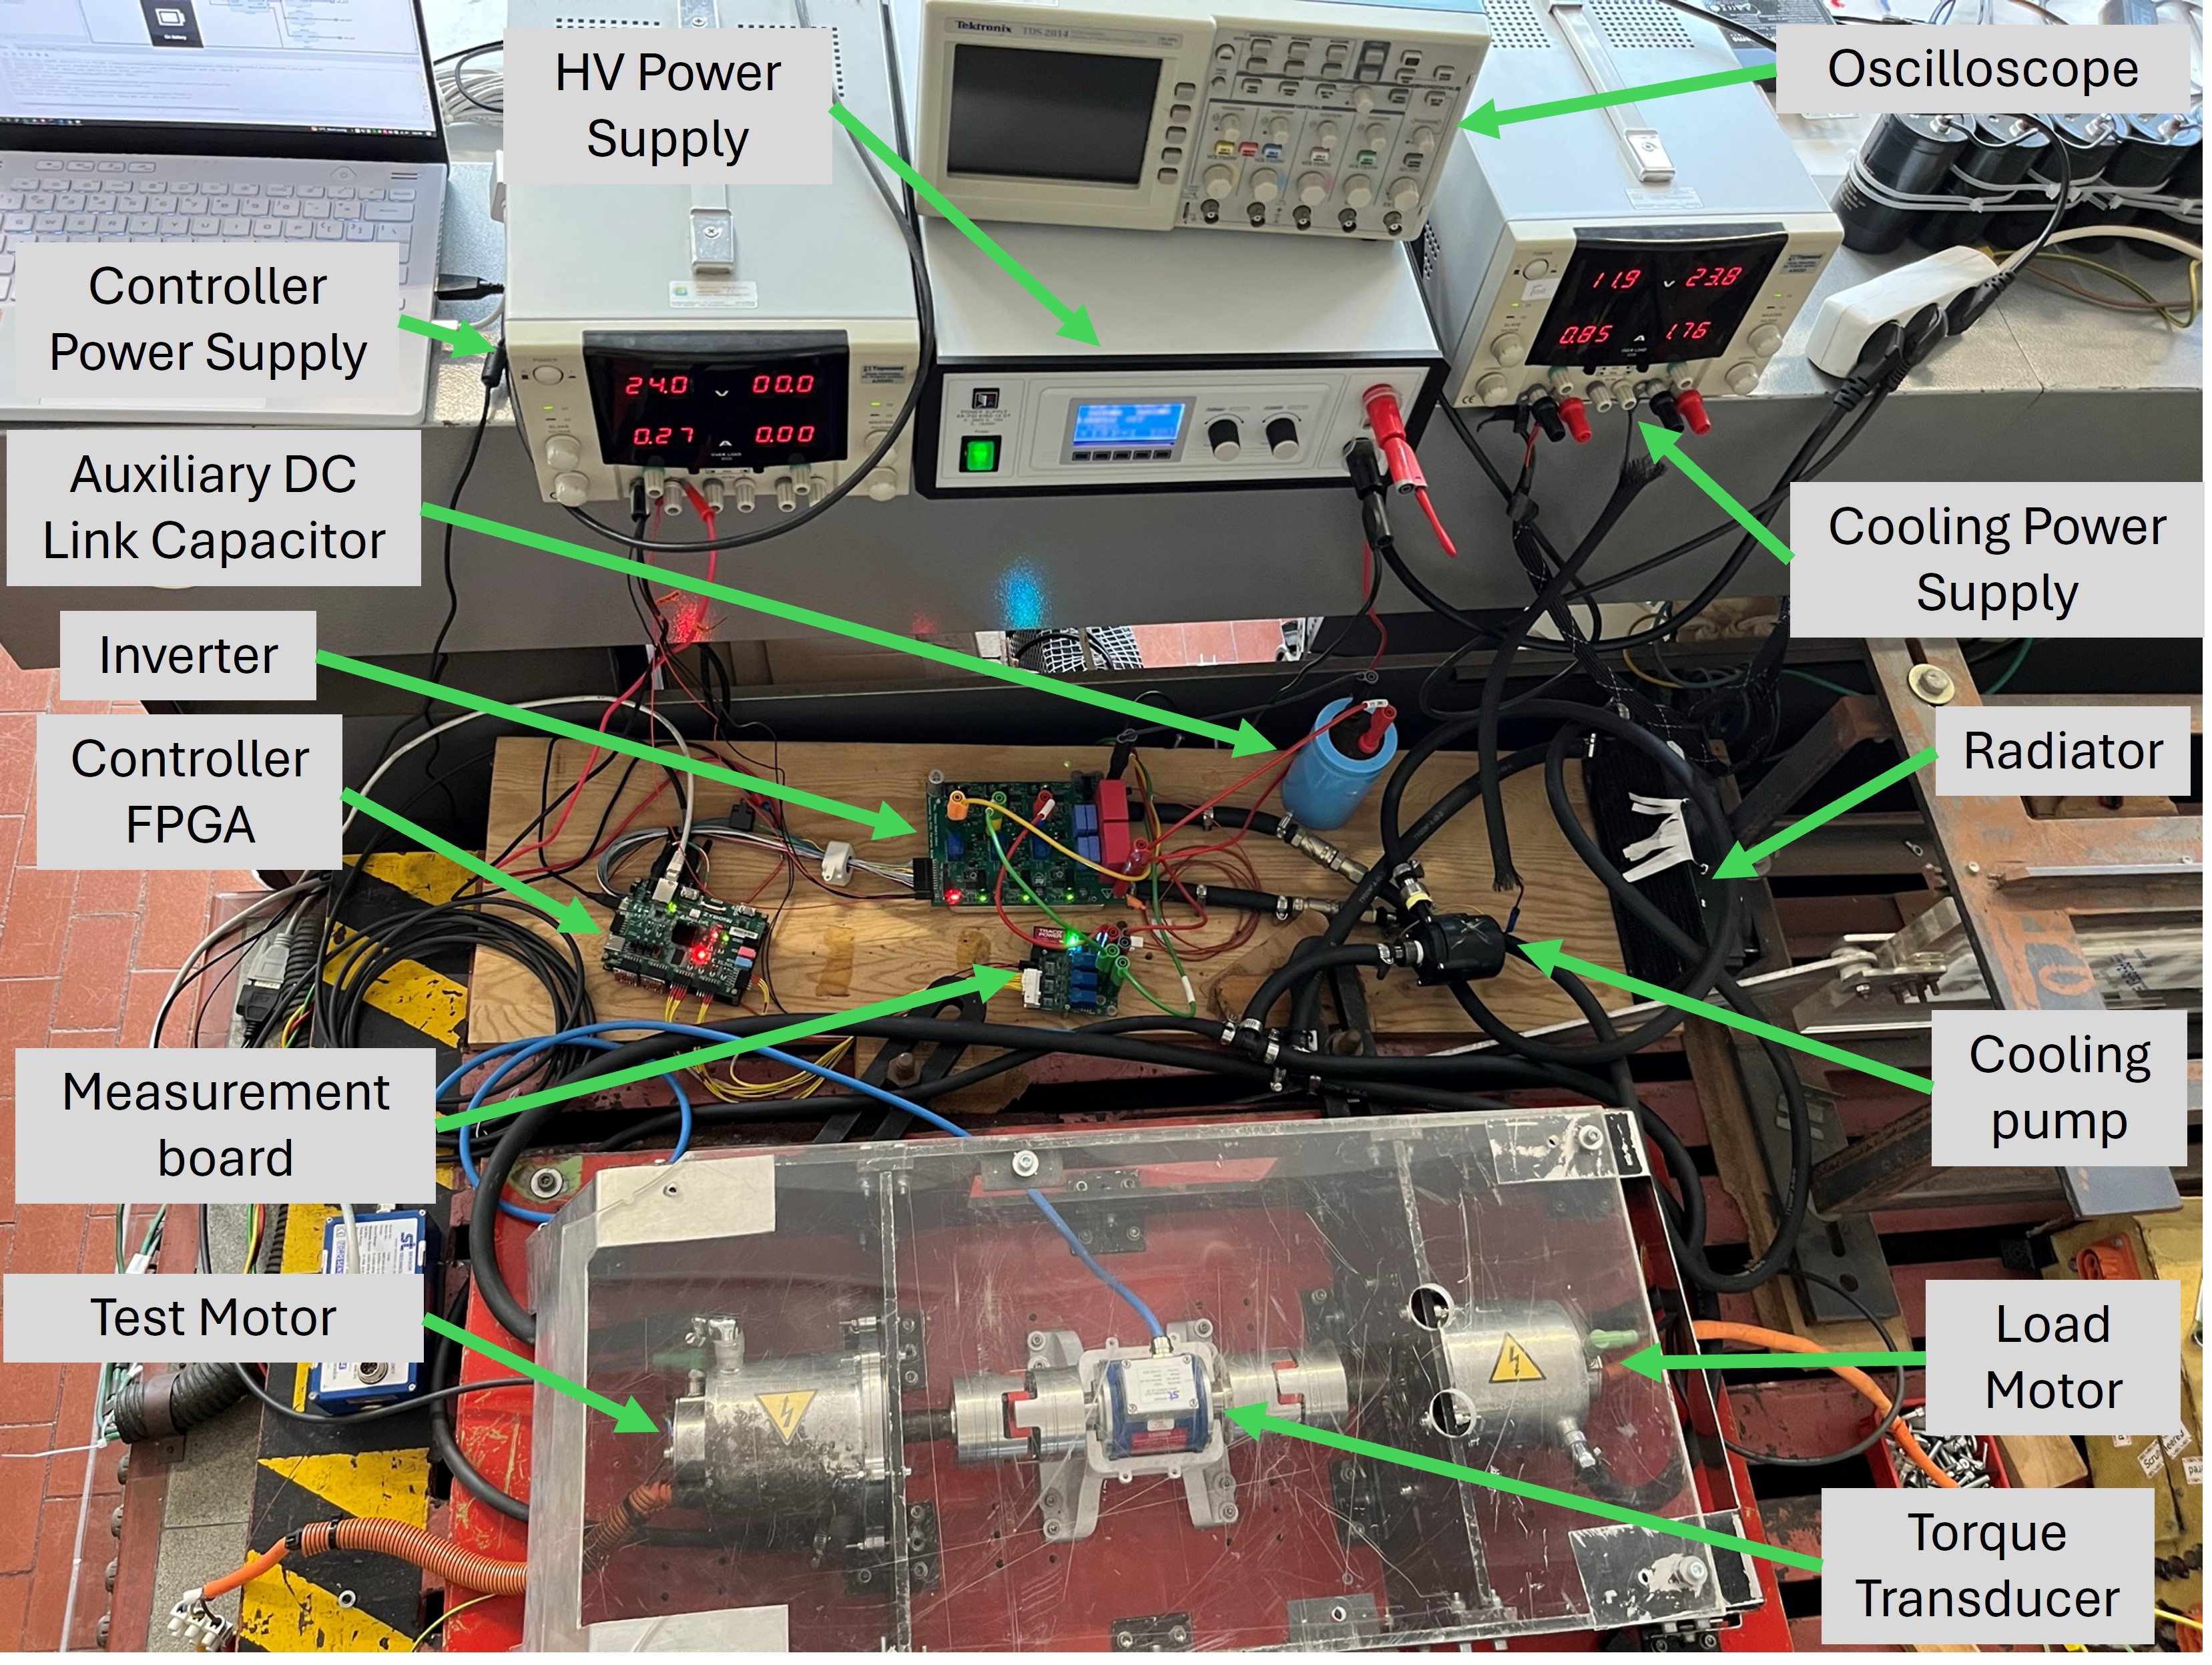
\includegraphics[width=.8\textwidth]{Figures/testbench_setup.jpg}
	\caption[Testbench setup.]{Testbench setup.}
	\label{fig:testbench_steup} %chktex 24
\end{figure}

First, a simple constant torque test was made to evaluate if the model was correctly calculating the generated torque. \Cref{fig:constant_tq} presents the torque estimated based on the motor parameters and the current measurements with the value measured with the ST transducer output. The current measurement from the developed measurement board had some outliers from \gls{emi}, so the currents and torque in this section were filtered using a moving median (8 samples) and if the sample is further than 2 \gls{mad}, then it is considered an outlier, thus it is replaced by the average of the closest 2 points.

\begin{figure}[!htb]
	\centering
	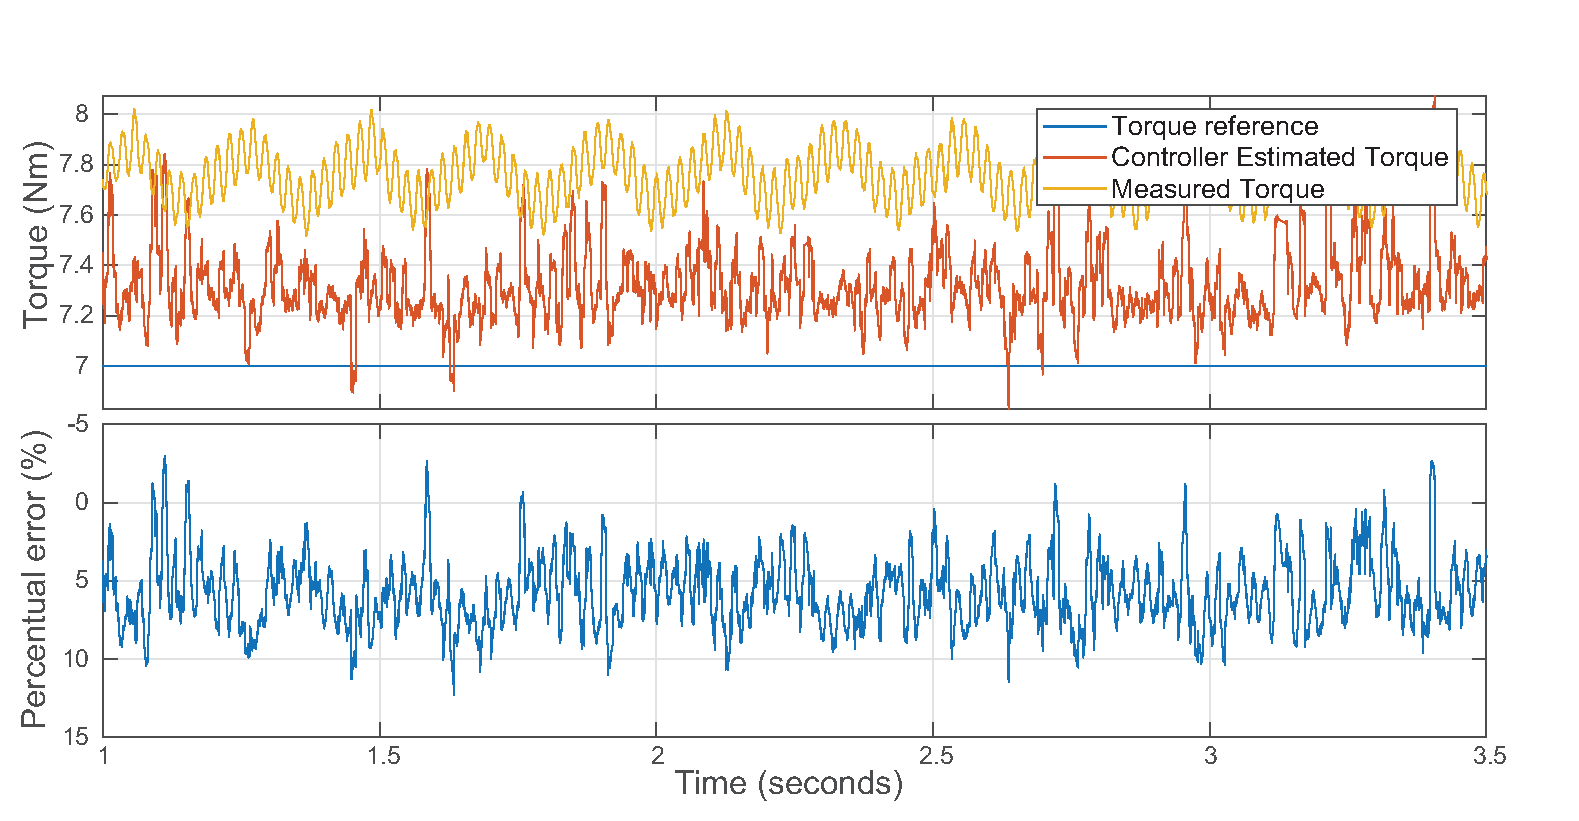
\includegraphics[width=0.8\linewidth]{Figures/constantTq.eps}
	\caption[Torque estimation vs Measured. In the bottom the percentual error between the measured and estimated torques is shown.]{Torque estimation vs Measured. At the bottom, the percentual error between the measured and estimated torques is shown.}
	\label{fig:constant_tq} %chktex 24
\end{figure}

The estimated torque is constantly smaller than the measured torque, with a difference of 0.5Nm. This difference is due to the motor parameters not being perfectly matched with the real motor, and the current measurements not being perfect. The difference between the estimated and measured torque is small enough to consider the model valid for the next tests.

With the torque estimation validated, the next step was to verify the currents on a steady state test, ideally, this would be done with nominal torque, but due to a limited maximum inverter current the motor was commanded to keep a constant torque of $7Nm$. To create a load, another motor was connected to the shaft and the motor phases were short-circuited, creating a load torque that changes with the speed, this resulted in the speed stabilizing at $269RPM$. The current was measured with the developed measuring board and with an oscilloscope probe (ELDITEST CP6550), while the torque was estimated by the control algorithm and compared with the simulation results. The simulation results were obtained by running the same model used for the controller implementation, with the same parameters and inputs. The results are presented in \Cref{fig:steady_state_curr}.
\begin{figure}[!htb]
	\begin{subfigmatrix}{2}
		\subfigure[Meausurement Board and Simulation measurements. The plot on top present values from the measurement board, while the bottom plot is from the simulation.]{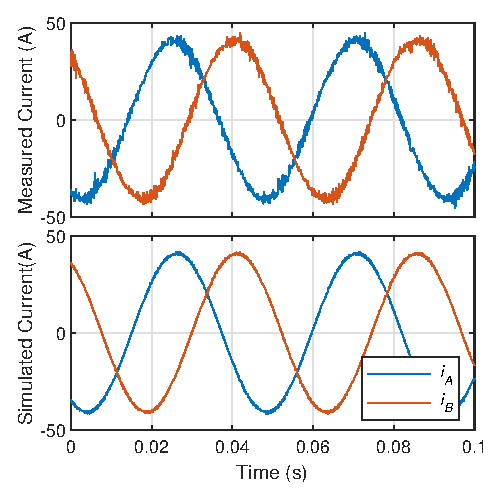
\includegraphics[width=0.47\linewidth]{Figures/const_curr_7NM.eps}\label{fig:steady_state_curr_sim_meas}}
		\subfigure[Osicloscope measurements. Channel 1 (in yellow) represents the line A current, while channel 2 (in blue) is the line B current]{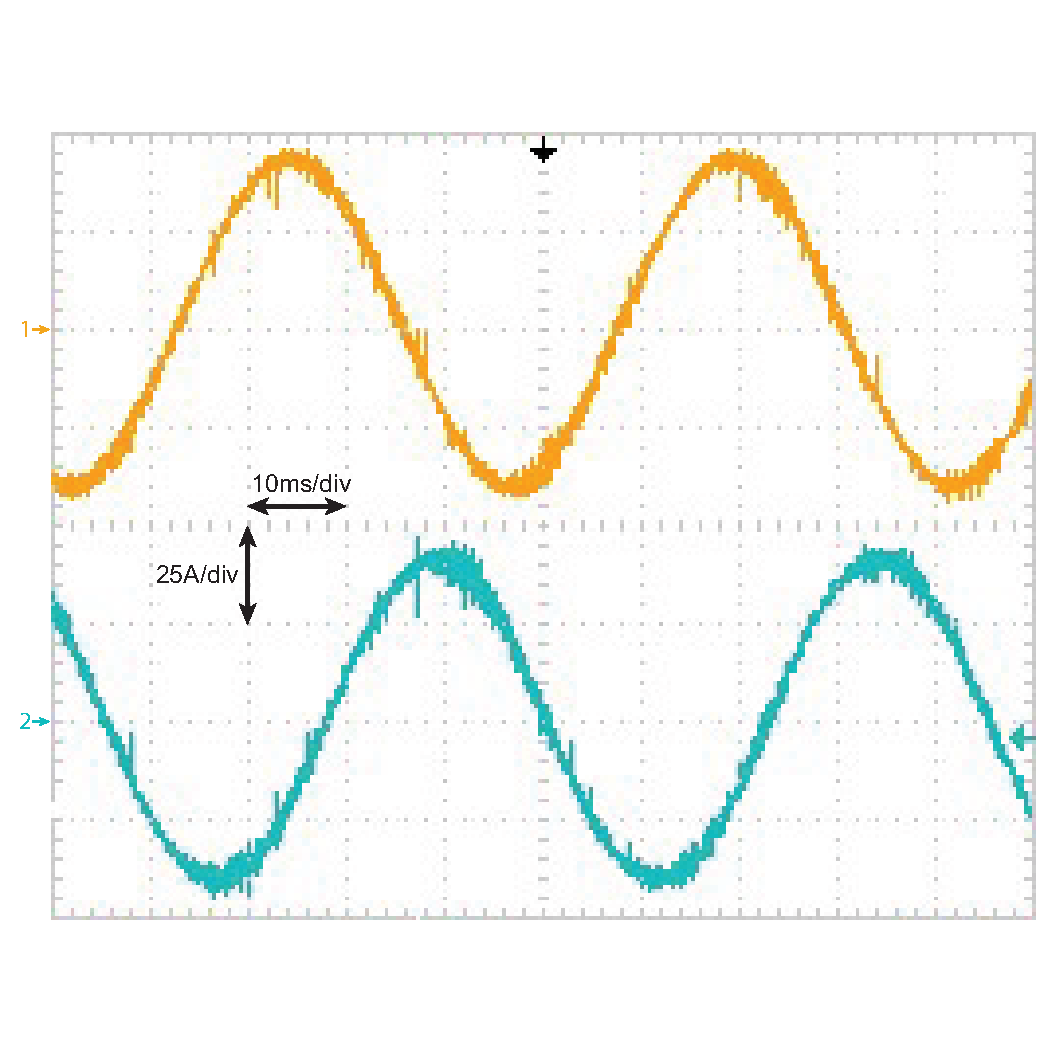
\includegraphics[width=0.52\linewidth]{Figures/const_curr_osc_7nm-01.eps}\label{fig:steady_state_curr_osc}}
	\end{subfigmatrix}
	\caption{Line currents measurements at steady state. Torque reference at $7Nm$ and rotor speed stable at $169RPMs$.}
	\label{fig:steady_state_curr} %chktex 24
\end{figure}

 The oscilloscope measurement was made with a probe that has a sensitivity of $20mV/A$. The results show that the current measured by the developed board is identical to the one from the oscilloscope probe, proving the system's accuracy. When comparing the measured currents with the simulation results, although they have the same form and amplitude, it is clear that the simulated curve is cleaner. This is backed by the \gls{thd} comparison, where the measured current has a \gls{thd} of $2.44\%$ and the simulated current has a \gls{thd} of $0.47\%$, both of them calculated to the 50th harmonic. This difference is due to inaccuracies in the measurements and parametrization. 
% While noisier, the measured current is still a great improvement over the previous control method, where the simulated current had a \gls{thd} of $1.65\%$.

Then a torque step response was applied with the motor at a standstill and with the same load as the constant current test. Once again it would be a good approach to use the nominal values but the inverter was a limitation so a reference of $7Nm$ was used. The currents presented in \Cref{fig:tq_step_fig} show an almost instantaneous dynamic response, transitioning to the specified amplitude without noticeable distortions. The oscilloscope currents are also very similar to the ones measured by the developed board, with the same form and amplitude. The simulation results are very similar to the measured ones, with the same form and amplitude, but the simulation is cleaner.  The difference between the measured and simulated currents is small enough to consider the model valid.
\begin{figure}[!htb]
	\begin{subfigmatrix}{2}
		\subfigure[Meausurement Board and Simulation measurements. The plot on top presents values from the measurement board, while the bottom plot is from the simulation.]{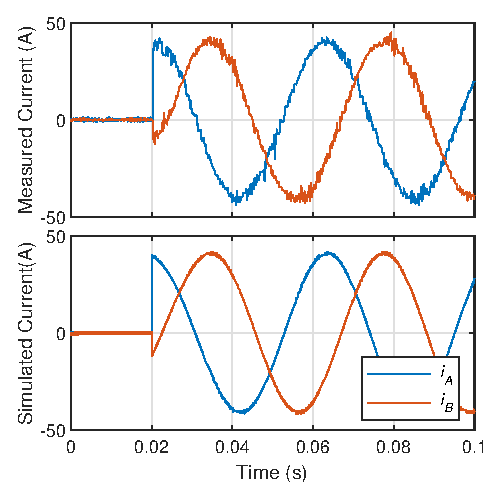
\includegraphics[width=0.47\linewidth]{Figures/tq_step_curr.eps}\label{fig:tq_step_curr}}
		\subfigure[Osicloscope measurements. Channel 1 (in yellow) represents the line A current, while channel 2 (in blue) is the line B current]{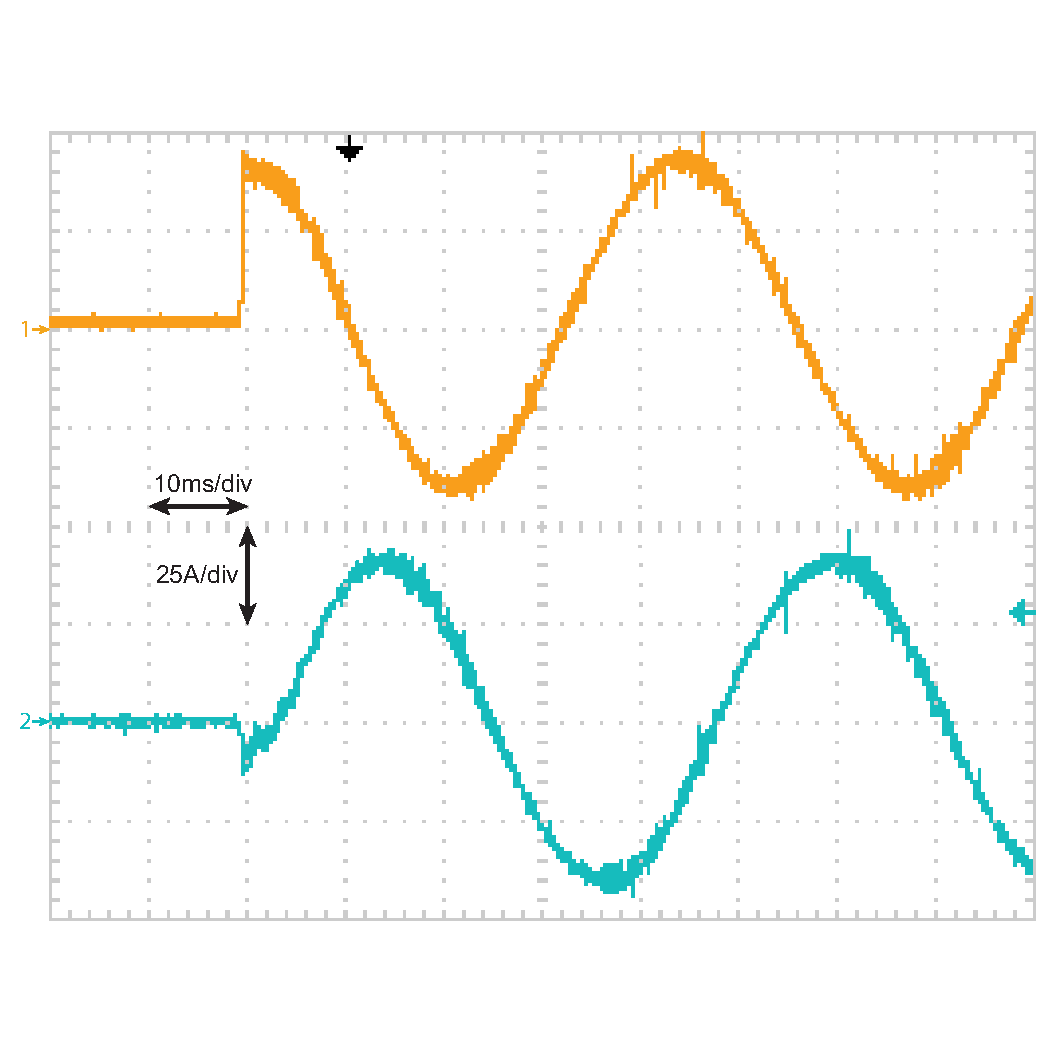
\includegraphics[width=0.52\linewidth]{Figures/tq_step_osc-01.eps}\label{fig:tq_step_osc}}
	\end{subfigmatrix}
	\caption{Line Current measurements with a reference torque step from $0$ to $7Nm$ at $0.02s$.}
	\label{fig:tq_step_fig} %chktex 24
\end{figure}



\Cref{fig:tq_step_response_time} shows the torque dynamic response to the step. The reduced sampling time creates significant uncertainty in the measurement, but it is possible to state that the torque rise time is less than 200 microseconds, which is a great improvement when compared with the current control method. The simulation results have a greater sampling rate showing that the rise time is smaller than 100 microseconds. An improved sampling frequency would allow for a better comparison between the simulation and experimental results.

\begin{figure}[!htb]
	\centering
	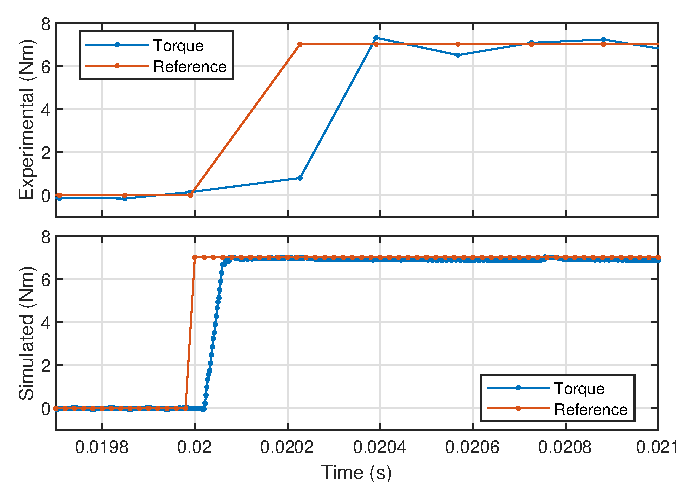
\includegraphics[width=0.55\linewidth]{Figures/Tq_step.eps}
	\caption[Torque reference follwoing with a step from $0$ to $7Nm$.]{Torque reference follwoing with a step from $0$ to $7Nm$. The upper plot presents the experimental data, while the bottom plot is from the simulation}
	\label{fig:tq_step_response_time} %chktex 24
\end{figure}

To compare the performance of the proposed method, a torque step was also applied to the current solution of the inverter and control strategy. The results presented in \Cref{fig:torque_step_comparison_FOC_MPC} show that as expected, the current solution is much slower than the proposed method, with a rising time of $30ms$ and a delay of $10ms$. When compared with the simulated values in \Cref{fig:rising_time_4_models} a difference can be seen in the overshoot value of the current method, which is not present in the experimental results.  That is due to the gains used on the PI current controller, which are not as aggressive as the ones used in the simulation. This also resulted in a slower rising time, as in the simulation it reached the $10Nm$ mark in half the time as the experimental results.

\begin{figure}[!htb]
	\centering
	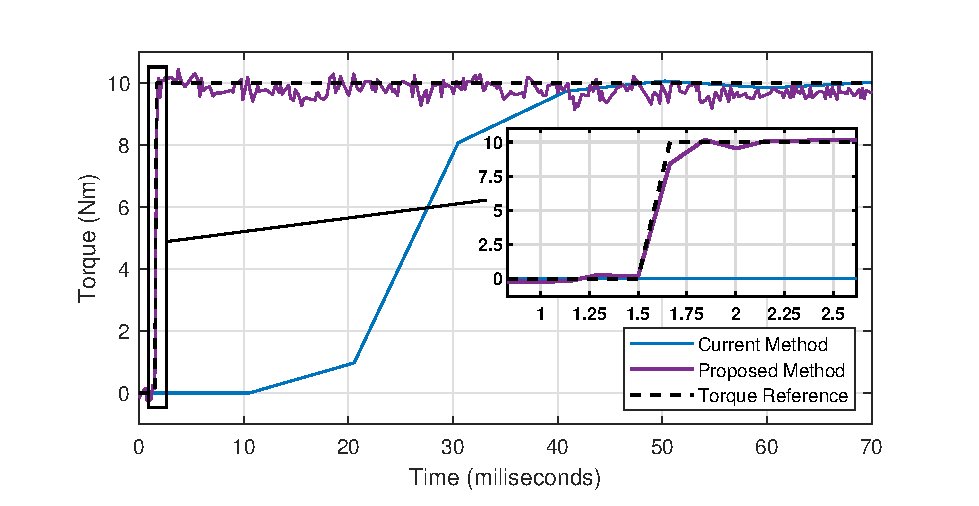
\includegraphics[width=0.7\linewidth]{Figures/Car_Tq_step.eps}
	\caption{Comparison of torque step response between the proposed method and the currently implemented method.}
	\label{fig:torque_step_comparison_FOC_MPC}%chktex 24
\end{figure}

The torque step response was repeated for several reference torque values, from $1$ to $10Nm$, to evaluate the tracking capabilities of the controller. The results presented in \Cref{fig:tq_step_response_multiple} show that the \gls{rush} is capable of tracking the reference torque independently of its magnitude. The rising time stayed constant throughout the steps, being smaller than the sampling time of $157\mu s$. It can also be seen that there is not a pronounced overshoot. 

\begin{figure}[!htb]
	\centering
	\begin{subfigmatrix}{3}
		\subfigure[$1Nm$]{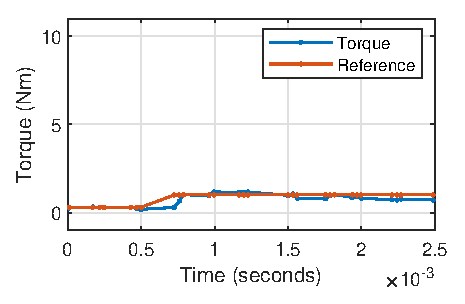
\includegraphics[width=0.31\linewidth]{Figures/torque_step_1Nm_tq.eps}\label{fig:torque_step_1Nm}}
		\subfigure[$3Nm$]{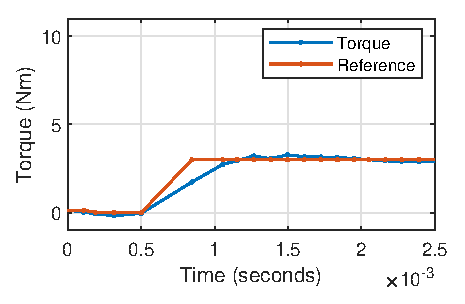
\includegraphics[width=0.31\linewidth]{Figures/torque_step_3Nm_tq.eps}\label{fig:torque_step_3Nm}}
		\subfigure[$5Nm$]{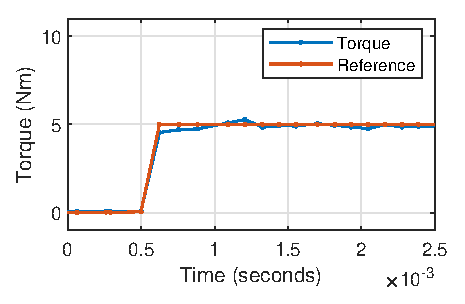
\includegraphics[width=0.31\linewidth]{Figures/torque_step_5Nm_tq.eps}\label{fig:torque_step_5Nm}}
	\end{subfigmatrix}
	\begin{subfigmatrix}{3}
		\subfigure[$6Nm$]{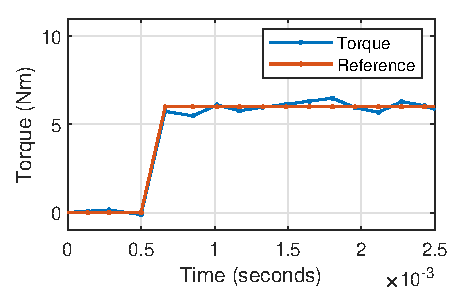
\includegraphics[width=0.31\linewidth]{Figures/torque_step_6Nm_tq.eps}\label{fig:torque_step_6Nm}}
		\subfigure[$7Nm$]{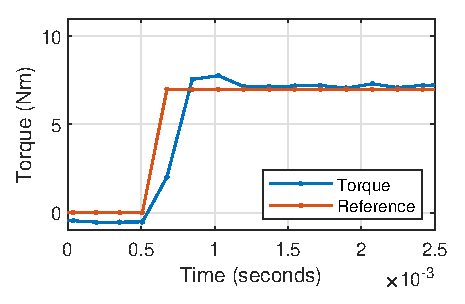
\includegraphics[width=0.31\linewidth]{Figures/torque_step_7Nm_tq.eps}\label{fig:torque_step_7Nm}}
		\subfigure[$8Nm$]{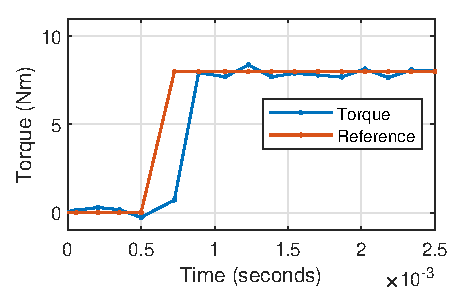
\includegraphics[width=0.31\linewidth]{Figures/torque_step_8Nm_tq.eps}\label{fig:torque_step_8Nm}}
	\end{subfigmatrix}
	\subfigure[$10Nm$]{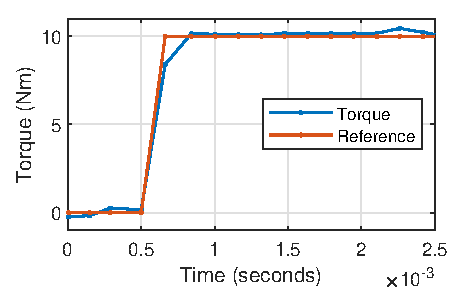
\includegraphics[width=0.31\linewidth]{Figures/torque_step_10Nm_tq.eps}\label{fig:torque_step_10Nm}}
	\caption{Torque step response for different reference torque values.}
	\label{fig:tq_step_response_multiple}
\end{figure}


To test the speed controller, an RPM step was applied with the motor at standstill and without load. In \Cref{fig:speed_step_fig} the rotor speed and the torque are presented. The speed controller was saturated to $\pm 5Nm$ to avoid overcurrents as the power supply was not able to constantly supply high currents. A small overshoot can be seen in the speed response, this is due to the exponential average filter that was implemented on the RPM measure. The filter reduced the bandwidth of the signal and when combined with high gains in the PI it produced some oscillations which can be improved with a less aggressive filter and a better-tuned PI controller. The \gls{rush} has great tracking capabilities, as shown by the torque graph, with the estimated torque overlaying the reference torque. The error between the torque reference and the estimated torque is shown in \Cref{fig:rpm_step_tq_error}, showing an average error of $0.05Nm$ and a peak error of $0.9Nm$.


\begin{figure}[!htb]
	\centering
	\subfigure[RPM reference and measured values.]{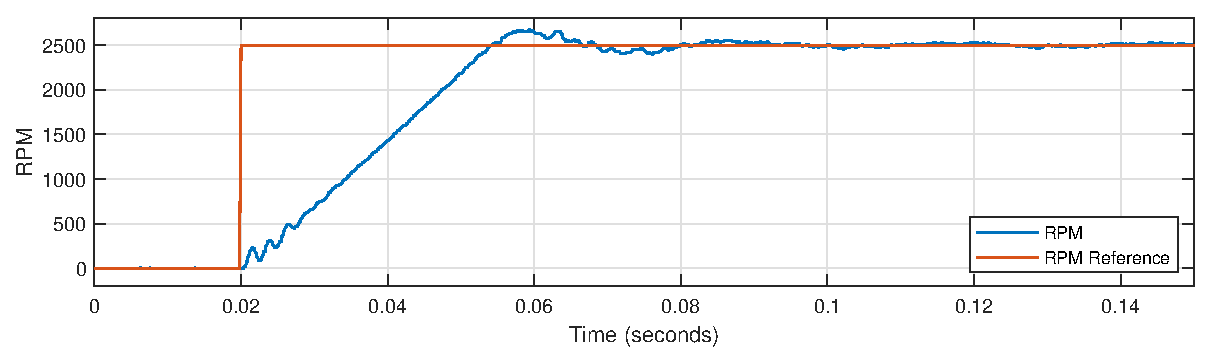
\includegraphics[width=0.8\linewidth]{Figures/rpm_step_rpm.eps}\label{fig:rpm_step_rpm}}
	\\
	\subfigure[Torque reference and measured values. The torque reference is derived from the speed controller but saturated to $\pm 5Nm$.]{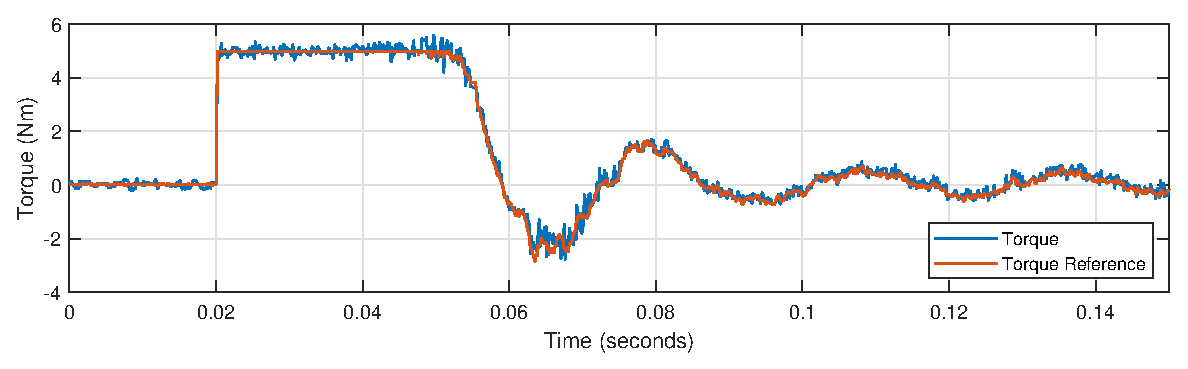
\includegraphics[width=0.8\linewidth]{Figures/rpm_step_tq.eps}\label{fig:rpm_step_tq}}
	\\
	\subfigure[Torque reference tracking error. ]{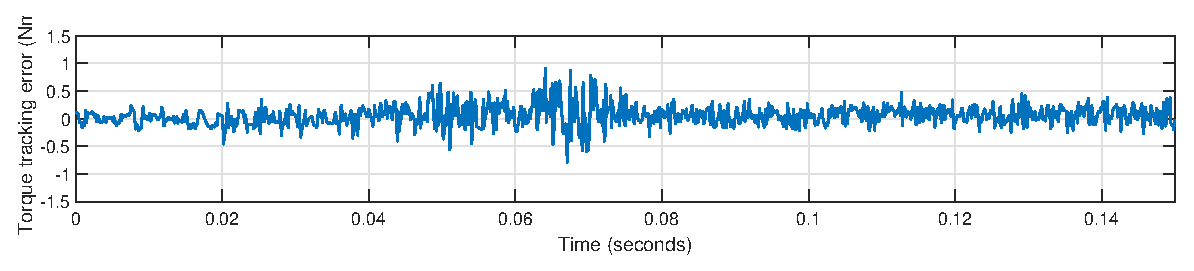
\includegraphics[width=0.8\linewidth]{Figures/rpm_step_tq_error.eps}\label{fig:rpm_step_tq_error}}
	\caption{RPM step from standstill to 2500RPMs.}
	\label{fig:speed_step_fig} %chktex 24
\end{figure}

A torque profile to simulate the driver's input was also tested and is presented in \Cref{fig:pedal_profile}. The controller fails to output the reference torque around $0.1s$ due to the power supply not being able to provide enough current, thus it switched from constant voltage to constant current output, reducing the available voltage to the inverter. Aside from this, the controller was able to follow the torque reference with a small error, averaging $0.04Nm$ and peaking at $1.6Nm$ if the period of the power supply shortage is discarded.
%  A small dependency on the speed can be seen in the torque tracking error, with the error slightly increasing with the rotor velocity. This is seen in the torque ripple increasing, due to the increased back \gls{emf} that requires the controller to increase the modulation index to keep the current amplitude, resulting in saturation

\begin{figure}[!htb]
	\centering
	\subfigure[Line Currents.]{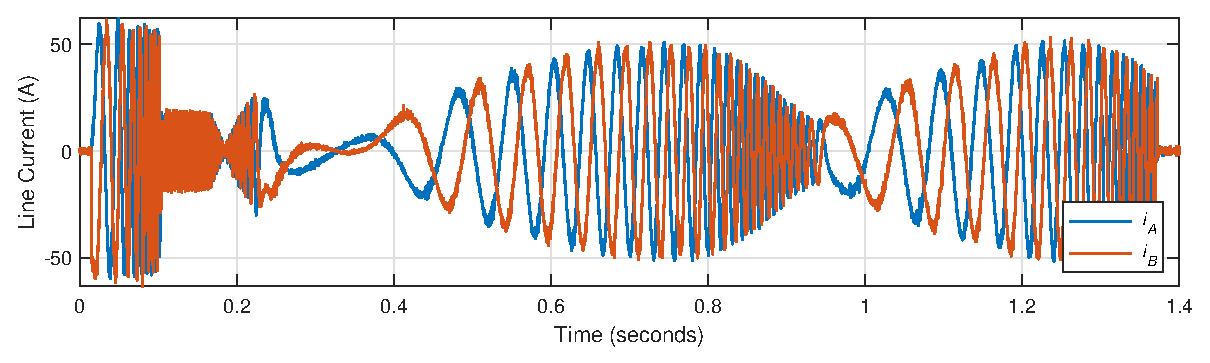
\includegraphics[width=0.85\linewidth]{Figures/pedal_profile_curr.eps}\label{fig:pedal_profile_curr}}
	\\
	\subfigure[Rotor speed.]{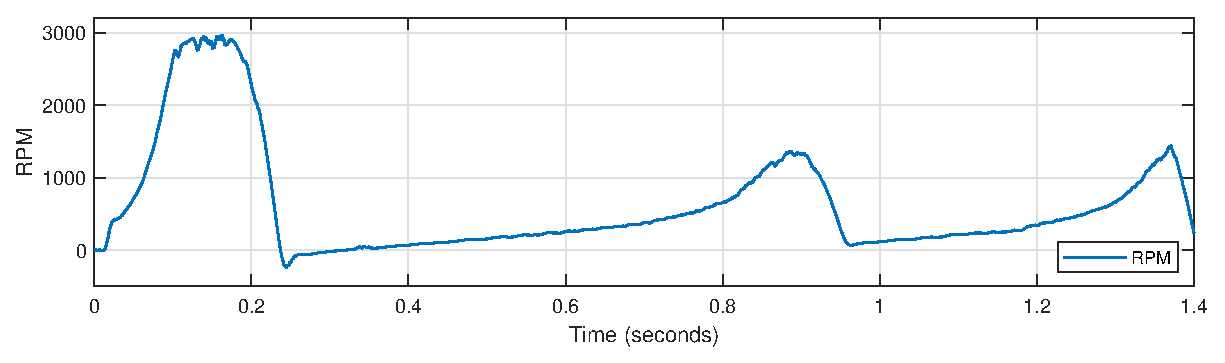
\includegraphics[width=0.85\linewidth]{Figures/pedal_profile_rpm.eps}\label{fig:pedal_profile_rpm}}
	\\
	\subfigure[Torque reference and measured values. The torque reference is derived from the speed controller but saturated to $\pm 5Nm$.]{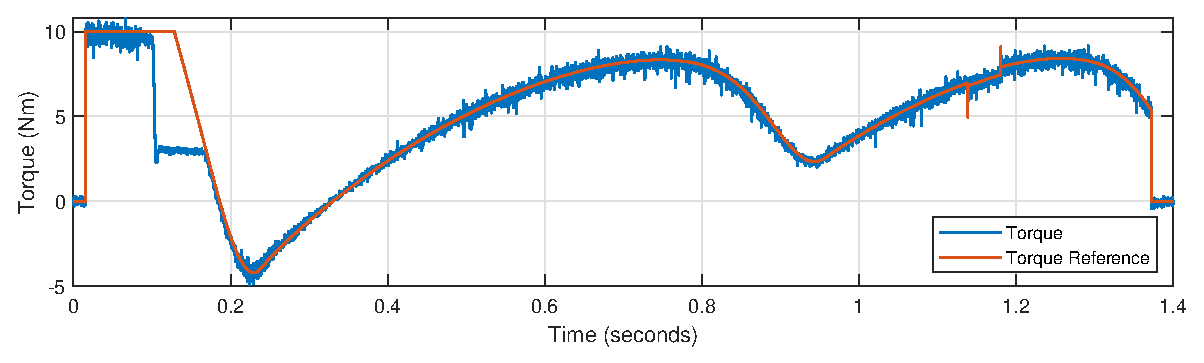
\includegraphics[width=0.85\linewidth]{Figures/pedal_profile_tq.eps}\label{fig:pedal_profile_tq}}
	\\
	\subfigure[Torque reference tracking error. ]{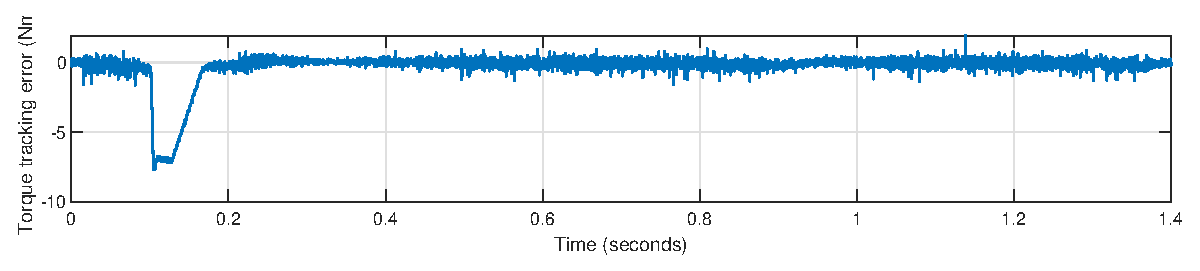
\includegraphics[width=0.85\linewidth]{Figures/pedal_profile_tq_error.eps}\label{fig:pedal_profile_error}}
	\caption{Pedal torque profile.}
	\label{fig:pedal_profile} %chktex 24
\end{figure}